The Belle II Analysis Software Framework (basf2) serves as the comprehensive software infrastructure for all data processing and analysis tasks within the Belle II experiment.
This framework handles the complete data processing chain, from the initial unpacking of raw detector data to high-level physics analysis, including simulation generation, event reconstruction and particle identification.
Basf2 is the successor to basf, the analysis software for the first Belle detector.

Basf2's architecture aims to ensure three principles: modularity, flexibility and performance.
Modularity is achieved through a component-based architecture where individual processing tasks are encapsulated in discrete modules that can be combined and reconfigured as needed.
This in turn enables the flexibility to support diverse analysis workflows, from detector calibration to complex physics measurements, utilizing configurable processing chains.
Performance considerations influence the choice of implementation languages and the framework's memory management strategies, ensuring efficient processing of the large volumes of data characteristic of modern high-energy physics experiments.

\subsubsection{Implementation Language}
The core data processing components, including all computationally intensive modules for reconstruction algorithms, are implemented in C++ (cf.\ Tab.\ \ref{tab:basf2-loc}).
C++ was chosen due to the performance requirements of processing millions of collision events, where execution speed and memory efficiency are of critical importance, especially in the case of the trigger systems (see Sec.\ \ref{sec:processing-pipeline}).

Python serves as the high-level interface and configuration language for basf2.
All user interactions with the framework, such as the creation of analysis workflows and module configurations, occur through Python scripts, commonly referred to as steering files.

This allows to harness both the computational performance of C++ and the user-friendly syntax of Python

\subsubsection{Code Organization and Architecture}
The basf2 software stack distinguishes between external dependencies and core components developed specifically for Belle II.
External components include third-party libraries and tools that provide foundational functionality, such as ROOT \cite{root} for data analysis and visualization or Geant4 \cite{geant4} for detector simulation.
These externals are maintained in a separate repository from the core basf2 code.

The basf2 core includes the Belle-II-specific software, implementing data structures and processing routines for the individual detector components and more general reconstruction and analysis steps. The following paragraphs further explain the architecture of the basf2 core.

\paragraph{Packages}
A package in basf2 represents a logical collection of related functionality, typically organized around a specific detector subsystem or analysis tasks.
Each package corresponds to a top-level directory in the basf2 repository and contains modules, utility functions and documentation related to its domain.

\paragraph{Modules}
A basf2 module represents a self-contained unit of code, usually implemented in C++, that performs a specific task within the data processing workflow.
Each module implements a standardized interface that defines five main lifecycle methods, governing its behavior during execution:
\begin{itemize}[topsep=0pt]
    \item \textbf{initialize}: invoked once before event processing begins to perform any necessary initialization such as setting up resources and allocating memory
    \item \textbf{beginRun} and \textbf{endRun}: called at the start and end of each data-taking run\footnote{%
        Run: a sequence of events with consistent detector conditions
    }, allowing modules to perform run-dependent initialization or finalization tasks, such as resetting run-specific monitoring histograms
    \item \textbf{event}: contains the main processing logic and is called once for each processed event, implementing the core functionality of the module
    \item \textbf{terminate}: called once after all events have been processed and typically handles cleanup tasks or final calculations
\end{itemize}

\paragraph{Paths}
A path in basf2 defines an ordered sequence of modules that will process each event in turn.
Conceptually, a path acts as a pipeline: each event is passed through the modules in the specified order, with each module performing its designated task (see Fig.\ \ref{fig:basf2-path-schema} for a visualization).
The path represents the complete workflow for a particular analysis or processing task, from initial data input to final output generation.
Paths are constructed programmatically in Python steering files by adding modules in the desired execution order, allowing users to create custom processing chains.

The path-based approach provides flexibility in creating data processing workflows, enabling complex processing pipelines with support for parallel processing and conditional path execution. 
For conditional path execution, specialized modules can modify the processing path based on individual event characteristics (cf.\ path branching in Fig.\ \ref{fig:basf2-path-schema}, Left).

\begin{figure}[h]
  \centering
  \begin{minipage}[c]{0.5\textwidth}
    \centering
    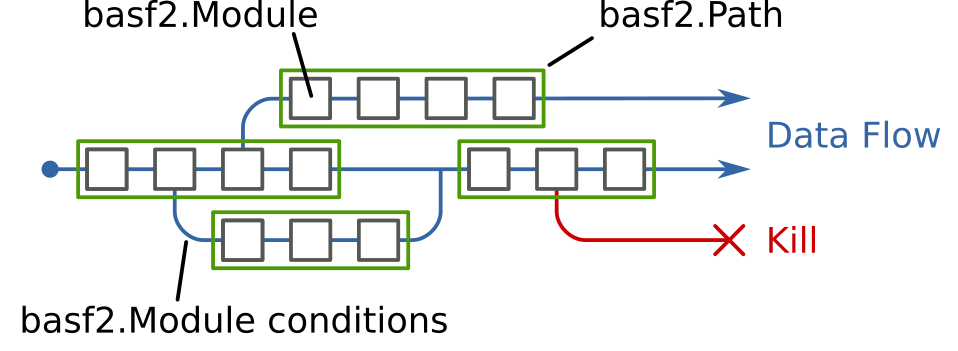
\includegraphics[width=\linewidth]{static/basf2-path-schema-left.png}
  \end{minipage}%
  \vrule%
  \begin{minipage}[c]{0.5\textwidth}
    \centering
    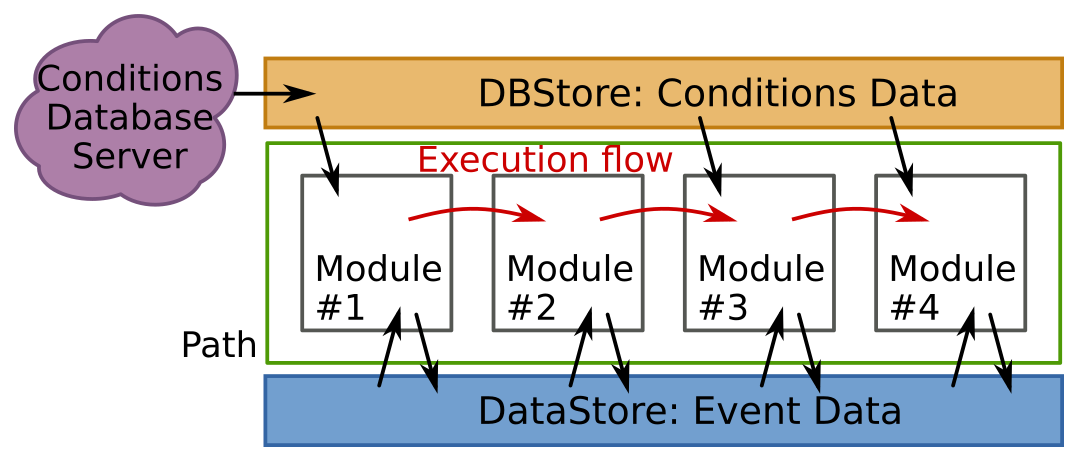
\includegraphics[width=\linewidth]{static/basf2-path-schema-right.png}
  \end{minipage}
  \caption{Schematic view of the processing flow in basf2 \cite{basf2-path-schema}}
  \label{fig:basf2-path-schema}
\end{figure}

\paragraph{DataStore and StoreArrays}
The DataStore serves as a globally accessible interface for sharing data objects between modules.
Instead of passing data directly between modules, all modules read from and write to the DataStore (see Fig.\ \ref{fig:basf2-path-schema}, Right). 
This is a key factor in maintaining the modularity of basf2's processing and avoids tight coupling between individual modules in a path.

StoreArrays represent collections of objects of the same type within the DataStore.
The framework provides functionality to model relationships between objects in different StoreArrays, such as the relationships between a track and the detector hits that it consists of.
This allows for efficient navigation between different levels of the reconstruction hierarchy.

\subsubsection{Detector Data Processing Flow}\label{sec:processing-pipeline}
\paragraph{Trigger System}
The necessity for event triggering, i.e.\ a pre-selection of observed events before they enter the processing and storage pipeline, stems from both technical and physics considerations.
From a technical perspective, the complete readout and storage of every collision event would overwhelm data acquisition systems and storage infrastructure.
From a physics standpoint, most collisions produce well-understood background processes that, while scientifically valid, are not relevant for the specific research goals of the Belle II experiment.
The trigger system enables filtering of interesting processes, such as B meson decays, that constitute the primary scientific targets of the experiment.

The trigger system operates in multiple stages to manage the high data rates from SuperKEKB collisions. 
The Level 1 (L1) trigger uses dedicated hardware to perform a (near) real-time selection of events based on reduced-resolution data from the CDC, ECL and KLM subsystems.
The downstream High Level Trigger (HLT) on the other hand performs full event reconstructions using basf2, allowing for complex physics-based selection criteria such as invariant mass requirements and vertex quality cuts.
The HLT's reliance on basf2 for event processing places high performance requirements on the framework's reconstruction algorithms, as any computational inefficiency directly impacts the experiment's data acquisition capabilities and overall trigger acceptance rates.

\paragraph{Reconstruction Pipeline}\label{par:reconstruction-pipeline}
The reconstruction process to transform raw detector signals into physics objects suitable for analysis includes the following main steps:
First, clustering algorithms group together signals from each detector subsystem that were likely produced by a common particle.
Track finding algorithms then use this information to identify particle trajectories through the central detector systems, combining hits from the PXD, SVD, and CDC to create a complete picture of each particle's path through the detector volume.
Subsequent track fitting procedures reconstruct the kinematic variables along these trajectories as precisely as possible.
The reconstructed tracks are then combined with additional data, such as energy deposits and timing information, to assign likelihoods for each track belonging to a certain particle species.
Finally, during high-level analysis, composite objects are created by combining reconstructed tracks and clusters according to physics hypotheses.